\begingroup
\titleformat{\chapter}{\normalfont\centering}{\chaptertitlename \thechapter}{14pt}{}
\titlespacing*{\chapter}{0pt}{-50pt}{0pt}

\chapter{Постановка задачи}
\label{cha:analysis}
%
% % В начале раздела  можно напомнить его цель
%

Перед началом научно-исследовательской работы был проанализирован ряд статей, посвященных применению методов глубокого обучения для следующих жанров игр: FPS (шутеры от первого лица) \cite{bergdahl2020augmenting}, прятки \cite{baker2019emergent}, а также аркадные и гоночные игры \cite{tufano2022using}.

\section{Среда}

В качестве среды для работы была выбрана платформа \textit{Gym} на языке Python \cite{Gym} по следующим причинам:
\begin{itemize}
	\item[--] в \textit{Gym} представлен ряд встроенных игр, которые можно использовать для тестирования моделей;
	\item[--] \textit{Gym} выступает в качестве посредника между игровой средой и агентом (моделью), выполняя нужные команды и собирая информацию о состоянии среды на каждом шаге.
\end{itemize}

Среди игровых сред, входящих в \textit{Gym}, была выбрана Lunar Lander v2 \cite{lunarlanderv2}. В ней игроку или агенту предлагается посадить лунный лендер (посадочный модуль) на заданную площадку, обозначенную флагами. Игра начинается с того, что центру масс модуля, находящегося наверху экрана, сообщается случайная сила. На каждом моменте времени можно привести в действие один трех двигателей: левый, правый или основной, либо ничего не делать. Игровой эпизод заканчивается, если лендер совершает посадку или покидает область видимости.

\section{Архитектура}

В научной литературе, прочитанной в рамках исследовательской работы, наиболее часто используемым алгоритмом являлся Deep Q-Network (DQN). Задача данного алгоритма "--- формирование функции полезности \(Q\), заданную следующим уравнением Беллмана: 
\begin{equation}
	Q(s_t, a_t) \leftarrow Q(s_t, a_t) + \alpha \cdot (r(s_t, a_t) + \gamma \cdot \max_a Q(s_{t+1}, a) - Q(s_t, a_t)),
\end{equation} где 
\begin{itemize}
	\item[--] \(s_t\) "--- состояние среды в момент времени \(t\); 
	\item[--]  \(a_t\) "--- действие агента, совершенное в момент времени \(t\);
	\item[--] \(\alpha \in (0, 1]\) "--- скорость обучения;
	\item[--] \(r(s_t, a_t)\) "--- награда, полученная при переходе из состояния \(s_t\) в состояние \(s_{t+1}\);
	\item[--] \(\gamma \in [0, 1]\) "--- дисконтирующий множитель; чем ближе он к единице, тем больше моделью будет учитываться награда в последующих состояниях.
\end{itemize}

Исследование агентом новых состояний и действий происходит благодаря $\varepsilon$-жадной стратегии принятия решений. Все они записываются в буфер воспроизведения (replay buffer), откуда на каждом шаге случайным образом выбирается партия из \(n\) кортежей вида \((s_t, a_t, r(s_t, a_t), s_{t+1})\).

В DQN используются две нейросети: одна отвечает за оценку \(Q\) для текущего состояния и обновляется на каждом шаге, когда как другая вычисляет оптимальное значения \(Q\) для последующего состояния (её веса изменяются периодически).

В качестве функции потерь была выбрана функция Хьюбера, т.~к. она является менее чувствительной к выбросам, нежели среднеквадратическая ошибка.

Для достижения большей стабильности при обучении использовалась модификация стандартного алгоритма DQN, называемая Dueling Double Deep Q-Network (D3QN) \cite{wang2016dueling,hasselt2016deep}. Кривые обучения такой модели представлены на Рисунке~\ref{fig:trainScore}

%\begin{figure}
%	\centering
%	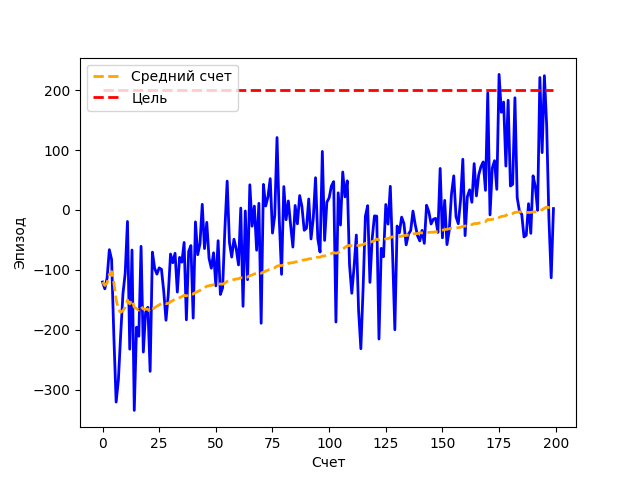
\includegraphics[width=\textwidth]{figures/d3qn_train_score}
%	\caption{Пример кривой обучения D3QN в среде Lunar Lander v2.}
%	\label{fig:trainScore}
%\end{figure}

\begin{figure}[ht]
	\begin{minipage}[b][][b]{0.49\linewidth}\centering
		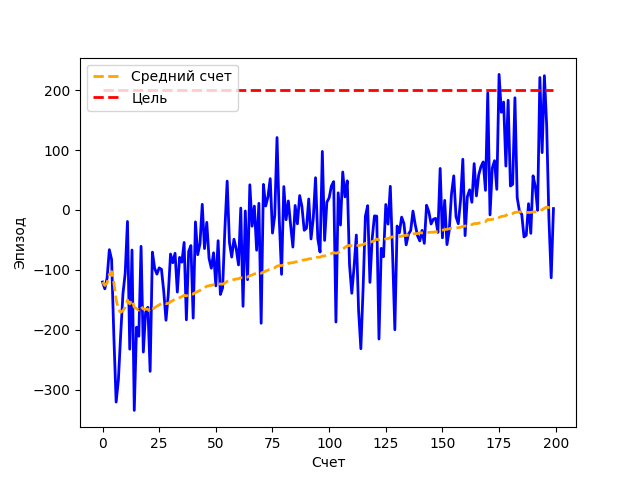
\includegraphics[width=\linewidth]{figures/d3qn_train_score1} \\ а)
	\end{minipage}
	\hfill
	\begin{minipage}[b][][b]{0.49\linewidth}\centering
		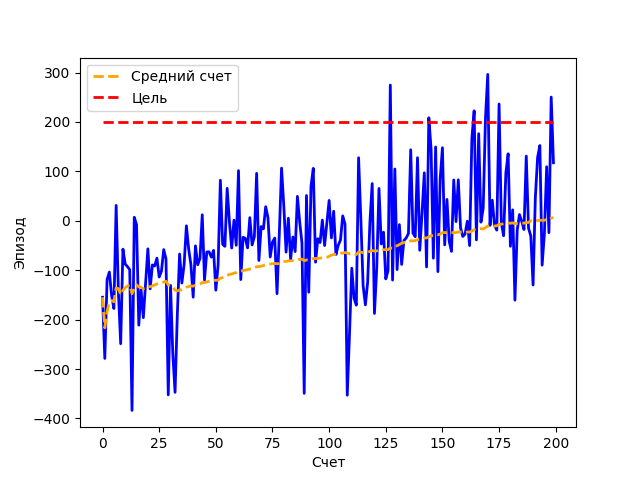
\includegraphics[width=\linewidth]{figures/d3qn_train_score2} \\ б)
	\end{minipage}
	\vfill
	\begin{minipage}[b][][b]{0.49\linewidth}\centering
		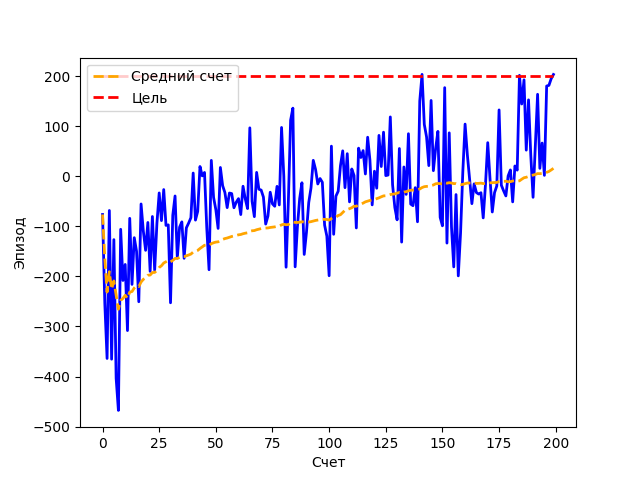
\includegraphics[width=\linewidth]{figures/d3qn_train_score3} \\ в)
	\end{minipage}
	\hfill
	\begin{minipage}[b][][b]{0.49\linewidth}\centering
		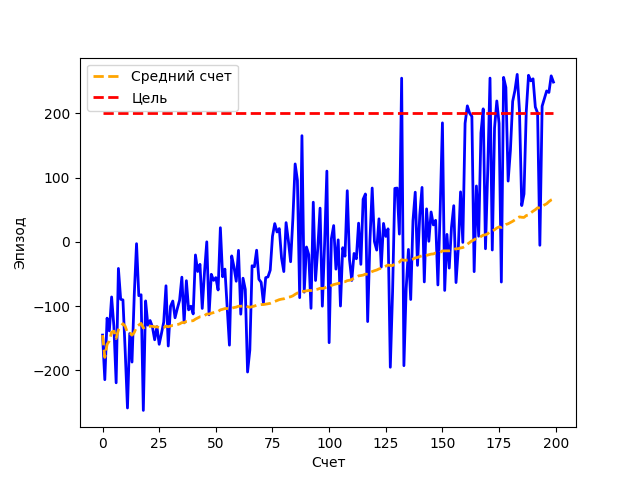
\includegraphics[width=\linewidth]{figures/d3qn_train_score4} \\ г)
	\end{minipage}
	\caption{Примеры кривых обучения алгоритма D3QN в среде Lunar Lander v2}
	\label{fig:trainScore}
\end{figure}

\endgroup

%%% Local Variables:
%%% mode: latex
%%% TeX-master: "rpz"
%%% End:
